%Dokumentklasse
\documentclass[a4paper,10pt]{scrreprt}
\usepackage[left= 2.5cm,right = 2cm, bottom = 4 cm]{geometry}
\usepackage[onehalfspacing]{setspace}
% ============= Packages =============

% Dokumentinformationen
\usepackage[
	pdftitle={Titel der Abschlussarbeit},
	pdfsubject={},
	pdfauthor={Euer Name},
	pdfkeywords={},	
	%Links nicht einrahmen
	hidelinks
]{hyperref}


% Standard Packages
\usepackage[utf8]{inputenc}
\usepackage[ngerman]{babel}
%\usepackage[T1]{fontenc}
\usepackage{fontspec}
\defaultfontfeatures{Mapping=text-text}
\setsansfont{Verdana}
\renewcommand*{\familydefault}{\sfdefault}
%\linespread{1.25}
\usepackage{graphicx, subfig}
\graphicspath{{img/}}
\usepackage{fancyhdr}
\usepackage{lmodern}
\usepackage{color}
\usepackage{hyperref}
\usepackage{float}
%\usepackage{caption}
% zusätzliche Schriftzeichen der American Mathematical Society
\usepackage{amsfonts}
\usepackage{amsmath}

%nicht einrücken nach Absatz
%\setlength{\parindent}{0pt}


% ============= Kopf- und Fußzeile =============
\pagestyle{fancy}
%
\lhead{}
\chead{}
\rhead{\slshape \leftmark}
%%
\lfoot{}
\cfoot{\thepage}
\rfoot{}
%%
\renewcommand{\headrulewidth}{0.4pt}
\renewcommand{\footrulewidth}{0pt}

% ============= Package Einstellungen & Sonstiges ============= 
%Besondere Trennungen
\hyphenation{De-zi-mal-tren-nung}

\setlength{\parindent}{0pt}


% ============= Dokumentbeginn =============

\begin{document}
%Seiten ohne Kopf- und Fußzeile sowie Seitenzahl
\pagestyle{empty}

\begin{center}
\begin{tabular}{p{\textwidth}}


%\begin{center}
%\includegraphics[scale=0.5]{img/logos.jpg}
%\end{center}


\\

\begin{center}
\LARGE{\textsc{
Entwicklung einer Webanwendung (Workshoppy) zur
Durchführung von Workshops in Echtzeit\\
}}
\end{center}

\\

\begin{center}
\textbf{\Large{Abschlussarbeit}}
\end{center}

\begin{center}
zur Erlangung des akademischen Grades\par
Bachelor of Science (B.Sc)
\end{center}

\begin{center}
an der\par
\end{center}

\begin{center}
\large{Hochschule für Technik und Wirtschaft Berlin\par
Fachbereich 4\par
Studiengang Angewandte Informatik \\}
\end{center}

\begin{center}
vorgelegt von
\end{center}

\begin{center}
\large{\textbf{Alongkorn Kiatmontri}} \\
\end{center}

\begin{center}
\large{(eingereicht am )}
\end{center}

\\

\\

\begin{center}
\begin{tabular}{lll}
\textbf{Erstprüfer:} & & Herr Prof. Jung, Th.\\
\textbf{Zweitprüfer:} & & Herr Andreas Flack (LB)\\
\end{tabular}
\end{center}

\end{tabular}
\end{center}

\addsec{Eidesstattliche Erklärung}
\label{erklaerung}

Hiermit versichere ich, die vorliegende Abschlussarbeit selbstständig und nur unter Verwendung der von mir angegebenen Quellen und Hilfsmittel verfasst zu haben. Sowohl inhaltlich als auch wörtlich entnommene Inhalte wurden als solche kenntlich gemacht. Die Arbeit hat in dieser oder vergleichbarer Form noch keinem anderem Prüfungsgremium vorgelegen.\\
\\[1.5cm]
Datum:	\hrulefill\enspace Unterschrift: \hrulefill
\\[3.5cm]

\newpage
\addsec{Danksagungen}
\label{danksagungen}




\addsec{Zusammenfassung / Abstract}
\label{sec:zusammenfassung}


\minisec{Abstract}
\label{abstract}


% Beendet eine Seite und erzwingt auf den nachfolgenden Seiten die Ausgabe aller Gleitobjekte (z.B. Abbildungen), die bislang definiert, aber noch nicht ausgegeben wurden. Dieser Befehl fügt, falls nötig, eine leere Seite ein, sodaß die nächste Seite nach den Gleitobjekten eine ungerade Seitennummer hat. 
\cleardoubleoddpage

% pagestyle für gesamtes Dokument aktivieren
\pagestyle{fancy}

%Inhaltsverzeichnis
\tableofcontents

%Verzeichnis aller Bilder
\listoffigures

%Verzeichnis aller Tabellen
\listoftables

\chapter{Einleitung}
\label{sec:einleitung}
Im ersten Kapitelabschnitt der Bachelorarbeit, wird auf die Motivation und die Zielsetzung eingegangen. Zusätzlich wird ein Überblick über den Aufbau der Arbeit aufgezeigt.

\section{Motivation}
\label{sec:motivation}
Beim Suchen und Finden von Lösungen, ungewöhnlichen Geschäftsideen, Innovationen oder um einzelne Projekte erfolgreicher zu machen, bereichert viele Menschen der Begriff Kreativität. Um die Kreativität zu fördern, braucht es Kreativitätstechniken, die dabei helfen, Ideen zu generieren und Einfälle zu sammeln.\bigskip

Der Klassiker und eine der bekanntesten unter allen Kreativitätstechniken ist das klassische Brainstorming. Sie wurde vom Amerikaner Alex Faickney Osborn erfunden und von Charles Hutchison Clark zur Ideenfindung innerhalb von Gruppen weiterentwickelt. 
(vgl. \cite{Ben.o.J.}) \glqq Er benannte das Brainstorming nach der Idee dieser Methode, nämlich using the brain to storm a problem (wörtlich: Das Gehirn verwenden zum Sturm auf ein Problem).\grqq{} \cite{Pas2012}\bigskip

Die Kreativitätstechnik Brainstorming gilt als eine der beliebtesten Methoden zur Ideenfindung und -sammlung neuer Geschäftsideen, Ideen für ein Projekt/Produkt oder auch zu einer vorhandenen bzw. gegebenen Problemstellung.\bigskip

Ziel des Brainstormings ist es, Denkblockaden auf der Suche nach neuen Ideen zu beenden. Diese Kreativitätstechnik wird häufig in Seminaren und Workshops angewendet, um die Gruppenarbeit effektiver und effizienter zu gestalten. Bei einer Brainstorming-Sitzung in einem Workshop kann jeder Teilnehmer auf die Ideen des anderen aufbauen und anknüpfen. Dadurch werden die Teilnehmer gegenseitig durch Ihre Ideen zu neuen Ideen angeregt, wodurch mehr Ergebnisse, als tatsächlich gebraucht, produziert werden.\bigskip

Eine häufig angewendete Methodik für die Ausarbeitung des Brainstormings in den Workshops ist es, sich Karteikarten oder Notizzettel zu nehmen, seine Ideen und Gedanken darauf zu schreiben und an eine Pinnwand (Flipchart, Whiteboard) anzubringen. Haben alle Teilnehmer Ihre Karteikarten an der Pinnwand angebracht, wird anschließend analysiert und darüber diskutiert. Am Ende der Besprechung werden die gesammelten Daten bewertet und anschließend von dem Moderator dokumentiert. Mit herkömmlichen analogen Workshops bedeutet das für den Moderator, dass er die Karteikarten auf der Pinnwand abtippen oder abfotografieren muss, um eine Dokumentation erstellen zu können. Da wir uns heutzutage in einem digitalen Zeitalter befinden und uns dieser neuen Welt nicht mehr entziehen können, gilt es, diesen Wandel als Chance zu begreifen, solche analogen Workshops zu digitalisieren, um dem Moderator eine Möglichkeit anzubieten, die Daten digital zusammenzufassen.

\section{Zielsetzung und Aufbau der Arbeit}
\label{subsec:zielsetzung}
Im Rahmen dieser Bachelorarbeit soll eine dynamische Webanwendung (Workshoppy) zur Durchführung von Workshops in Echtzeit entwickelt werden, die das klassische Brainstorming digitalisieren und effektiver machen soll. Die Webanwendung soll künftig in den Workshops genutzt werden und muss die Funktionen bieten, welche mehrere Personen (Teilnehmer) über Ihre Endgeräte (Smartphone, Laptop oder Tablet) ihre Ideen abgeben können. Dabei werden die eingebrachten Ideen der Teilnehmer in Echtzeit auf einer großen Leinwand (Beamer) präsentiert. Der Moderator soll anschließend die Möglichkeit erhalten, die Ergebnisse digital zusammenzufassen. Die Zusammenfassung soll auch als PDF-Datei exportiert werden können. Bei der Konzeption der Webanwendung ist zu beachten, dass eine benutzerfreundliche Darstellung für die Anwender gewährleistet ist.\bigskip

Die vorliegende Arbeit ist wie folgt aufgebaut: Das Kapitel \textbf{\ref{sec:grundlagen}} stellt vorab ein Überblick über einige grundlegende Begriffe vor. Der Begriff Responsive Webdesign, AJAX-Technologie und Rich Internet Applications (RIA) werden besprochen. Anschließend wird der Thin Client und Thick Client beschrieben. Das Kapitel \textbf{\ref{sec:analyse}} beschäftigt sich zunächst mit dem Stand der Technik. Die Anforderung zur Webanwendung wird dabei analysiert und konzipiert. In diesem Kapitel werden vor allem die funktionale, nicht-funktionale Anforderungen sowie die Muss- und Kann- Anforderungen ermittelt. Aufbauend auf den Ergebnissen der Anforderungsanalyse erfolgt in Kapitel \textbf{\ref{sec:design}} eine ausführliche Beschreibung über den Entwurf der Benutzeroberfläche (GUI) der Webanwendung. Danach wird das Design der GUI entworfen. Im Kapitel \textbf{\ref{sec:implementierung}} wird zunächst die zu verwendenden Webentwicklungswerkzeuge vorgestellt. Anschließend beschäftigt sich dieses Kapitel hauptsächlich mit der Implementierung der Webanwendung. Nach der Implementierung wird das Endergebnis im Kapitel \textbf{\ref{sec:bewertung}} anhand eines Fragebogens bewertet. Zum Schluss wird es im Kapitel \textbf{\ref{sec:schluss}} die erarbeiteten Ergebnisse zusammengefasst, sowie Ideen für zukünftigen Erweiterungen der entwickelten Webanwendung diskutiert.


\chapter{Anforderungsanalyse und Konzeption}
\label{sec:anforderungsanalyse}
Dieses Kapitel befasst sich mit der Anforderungsanalyse und Konzeption der Webanwendung. Dazu werden zunächst eine allgemeine Struktur festgelegt, wie das Projekt systematisch aufgebaut sein soll.
\\

Anschließend wird der aktuelle Zustand (Ist-Analyse) des Projektes ermittelt. Anhand dieser Ist-Analyse erfolgen die funktionalen und nicht funktionalen Anforderungen an die zu entwickelnde Webanwendung. Am Ende wird die Architektur der Webanwendung erklärt.


\section{Projektstruktur}
\label{sec:projektstruktur}
Nach Definition der DIN (Deutsches Institut für Normung e.v., 2009) 69901-5:2009 ist der Projektstrukturplan die \textit{“ [...] vollständige hierarchische Darstellung aller Elemente (Teilprojekte, Arbeitspakete) der Projektstruktur als Diagramm oder Liste.”}
\\

Auf der oberste Ebene steht das Projekt. Eine Ebene darunter die Teilprojekte oder Teilaufgaben, darunter schließlich die Arbeitspakete. 
Der Projektstrukturplan (Abbildung 2.1) entspricht dem typischen sequentiellen Vorgehensmodell zur Softwareentwicklung einschließlich der Entwicklung der Webanwendung.

\begin{figure}[H]
  \centering  
  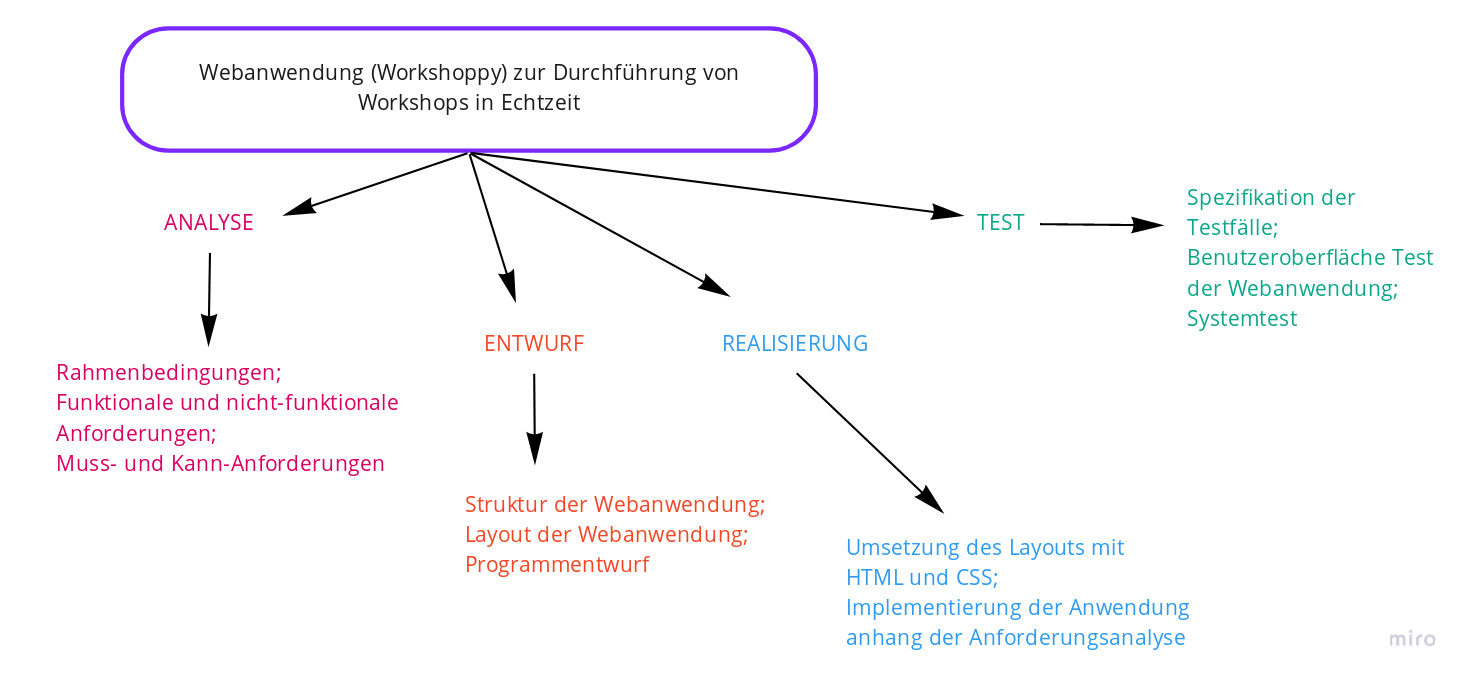
\includegraphics[scale=0.3]{img/Projektstrukturplan.jpg}
  \caption{Projektstrukturplan [Quelle: eigene Abbildung]}
  \label{fig:projektstrukturplan}
\end{figure}

\newpage
Eine Analyse von funktionalen und nicht-funktionalen Anforderungen sowie die Muss- und Kann-Anforderungen wird in der ersten Phase untersucht. Anhand dieser Analyse wird die Struktur und ein passendes Layout der Webanwendung erstellt. Der daraus entstehende Entwurf wird technisch in eine Webanwendung umgesetzt und am Ende getestet.

\section{Ist-Analyse}
\label{sec:ist-analyse}
Bei der Projektvorstellung wurde in der Firma zunächst über den Zustand der aktuellen Lösung für die Durchführung von Workshops gesprochen.
\\

Neben dem Brainstorming wird häufig das Mind-Mapping als Methode zur Ideenfindung, Problemlösung und Kreativitätssteigerung eingesetzt.  Eine Mindmap\footnote{auf deutsch: die Gedankenlandkarte} oder auch Mind-Mapping genannt, ist in der Regel mit dem Brainstorming verwandt. In der Abbildung \hyperref[sec:mind-map]{\textbf{\ref{fig:mind-map}}} wird diese Methode grob dargestellt. Das Hauptthema oder das Schlüsselwort befindet sich als Knoten kreisförmig in der Mitte. Um das Thema herum wird alles in Form von Hauptästen notiert. Man schreibt auf jeden Hauptast ein Schlüsselwort auf. Verbunden werden sie zum Hauptthema mit Linien. Die Hauptäste bilden die ersten Gedankengänge. Von jedem Hauptast zweigen weitere Nebenäste mit Begriffen ab.
\\

Bis jetzt existieren bereits mehrere webbasierte Mindmapping-Tools, mit denen man kostenlos Mindmaps erstellen, visualisieren und mit anderen in Echtzeit kollaborieren kann. Bei der Durchführung von Workshops gilt das Mindmapping aktuell als das idealste Format zum Brainstormen.
\\

Nach der Betrachtung der aktuellen Lösung fällt das Fazit des Unternehmens folgendermaßen aus: Die Mindmaps sehen auf den ersten Blick unübersichtlich und verschachtelt aus. Sie können sehr schnell ihre Übersichtlichkeit verlieren, wenn verschiedene Schlüsselwörter in Beziehung stehen. Es ist außerdem sehr zeitaufwendig, eine Mindmap exakt nach den Regeln zu erstellen. Mindmaps sind eher für den individuellen Gebrauch geeignet, da die verwendeten Schlüsselbegriffe und die Strukturierungen häufig für andere Personen unverständlich sind.
Es wird eine alternative Lösung benötigt, um dieses Problem benutzerfreundlicher und vor allem die Durchführung von Workshops effektiver zu gestalten.  

\begin{figure}[H]
  \centering  
  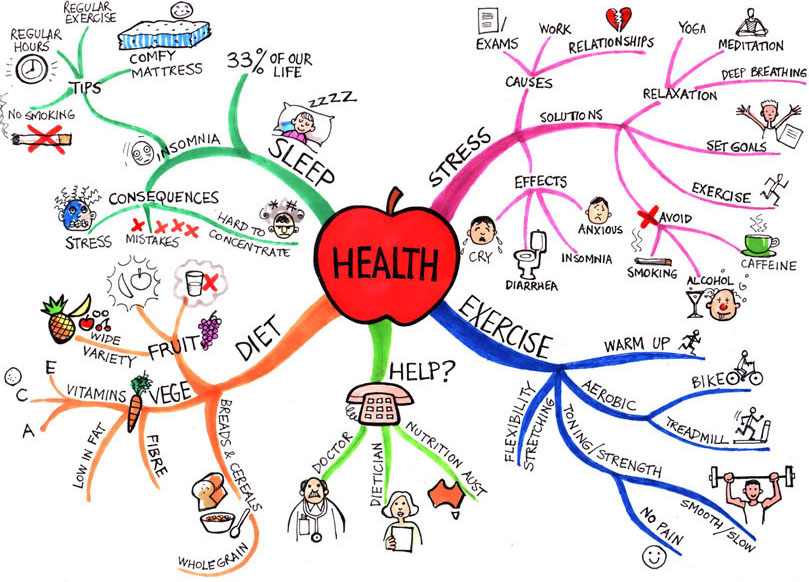
\includegraphics[scale=1.7]{img/health-mindmap}
  \caption{Beispiel einer Mind-Map\newline [Quelle: Learning Fundamentals: Student Study Techniques by Jane Genovese, Figure 4: Health mindmap. Online im Internet: URL: https://learningfundamentals.com.au/resources/\newline (Stand 11.07.2019)]}
  \label{fig:mind-map}
\end{figure}

\section{Anforderungsanalyse}
\label{sec:anforderungsanalyse}
Dieses Kapitel umfasst die grundlegende Anforderungen dieser Bachelorarbeit. Die Anforderung wird in funktionale und nicht- funktionale Anforderungen aufgeteilt. 
\\

Eine funktionale Anforderung wird nach der Definition aus dem Buch \cite{Balzert2010} die gewünschte Funktionalität des Systems bzw. eines Produkts beschrieben. 
Die nicht-funktionale Anforderungen sind Anforderungen, die für die Nutzung des Systems wichtig sind. Außerdem wird eine Muss- und Kann-Anforderung formuliert, welche für das Projekt oberste Priorität hat und welche eher zweitrangig ist.

\subsection{Funktionale Anforderungen}
\label{sec:funktionale anforderungen}
Aus den Unternehmensanforderungen lassen sich folgende funktionale Anforderungen ableiten.

\subsubsection*{Startseite}
Die Startseite der Webanwendung ist die Eingangsstelle für eine moderierende Person, nachdem diese sich bei der Anwendung angemeldet hat. Er kann auf dieser Seite neue Workshops erstellen, sie bearbeiten sowie löschen. Jeder Workshop hat einen Titel und wird in einer Datenbank gespeichert. Die erstellten Workshops werden nacheinander aufgelistet. Auf der Startseite soll außerdem eine Liste der beendeten Workshops anzeigen. In dieser Liste sind die Workshops, die von der moderierenden Person vorher beendet wurden. Das Datum und die Uhrzeit, an dem die Workshops beendet wurden, soll ebenfalls ausgegeben werden. Außerdem soll jeder beendete Workshop einen Button besitzen, der die Ergebnisse des Workshops anzeigt. 

\subsubsection*{Controller-Seite}
Der ausgewählte Workshop soll zur Controller-Seite führen. Diese Seite beinhaltet unter anderem den Titel vom ausgewählten Workshop und eine Liste der Sessions. Die Sessions können vom Moderator erstellt werden. Er soll sie auch bearbeiten und löschen können. Beim Erstellen einer neuen Session soll neben den Titel auch eine Frage, die behandelt wird, angegeben werden. Die Frage wird als Pflichtfeld gekennzeichnet. Die Sessions werden ebenfalls wie bei den Workshops in einer Datenbank gespeichert. Beim Bearbeiten einer Session soll der Moderator neben Titel- und Fragenänderung auch als Option Kategorien zu dieser Session hinzufügen können.
\\ 

Eine Session versteht sich als eine Sitzung zur Ideenfindung und -sammlung, um Lösungen für eine Problemstellung zu finden. Der Moderator kann zu jedem Workshop mehrere Sessions erstellen.
\\

Jede Session auf der Controller-Seite eines ausgewählten Workshops muss drei Buttons enthalten, die der moderierenden Person folgende Funktionen anbieten:
\begin{itemize}
\item Session starten-Button:
\begin{itemize}
\item um Lösungen und Ideen für eine Problemstellung zu sammeln, muss die Session gestartet werden. Hat die moderierende Person eine Session gestartet, soll automatisch die Präsentation-Seite aufgerufen werden. Während eine Session läuft, sollte dieser Button bei den anderen Sessions deaktiviert sein.
\end{itemize}
\item Eingabe beenden-Button:
\begin{itemize}
\item beendet die Funktion zur Dateneingabe seitens der Teilnehmer. Auf der Präsentation-Seite soll nach dem Betätigen dieses Buttons ein Button zur Erstellen von Kategorien freigeschaltet werden.
\end{itemize}
\item Session beenden-Button:
\begin{itemize}
\item beendet die gestartete Session. Die Ergebnisse sollen anschließend in einer Datenbank gespeichert werden.
\item reaktiviert die zuvor deaktivierten Session starten-Buttons.
\end{itemize}
\end{itemize}

Folgenden Buttons müssen ebenfalls auf der Controller-Seite zur Verfügung stehen:
\begin{itemize}
\item Client-Button:
\begin{itemize}
\item zeigt die Teilnehmer-Seite. Sie stellt den Teilnehmern die Funktionen für Dateneingabe bereit.
\end{itemize}
\item Präsentation-Button:
\begin{itemize}
\item zeigt die Präsentation-Seite. Die Präsentation-Seite wird über dem Beamer angezeigt und präsentiert die eingegebenen Daten von allen Teilnehmern in Echtzeit.
\end{itemize}
\item Ergebnisse-Button:
\begin{itemize}
\item ruft die Ergebnisse-Seite auf. Die Ergebnisse von allen Sessions eines ausgewählten Workshops werden auf der Seite in Form einer Tabelle präsentiert.
\end{itemize}
\item Workshop Beenden-Button:
\begin{itemize}
\item beendet den ausgewählten Workshop und führt den Moderator zu Startseite zurück. Der Workshop soll sich anschließend in der Liste der beendeten Workshops befinden.
\end{itemize}
\end{itemize}

Die Controller-Seite eines ausgewählten Workshops soll außerdem dem Moderator die Funktion anbieten, die es ihm erlaubt, den Teilnehmer eine Einladungsmail zur Teilnahme am Workshop zu senden.

\subsubsection*{Teilnehmer-Seite}
Die Teilnehmer-Seite soll jedem Teilnehmer am Workshop die Funktion zur Dateneingabe zu einer gestarteten Session bereitstellen. Der Teilnehmer muss die Möglichkeit haben, sich mit seinem Namen einloggen zu können. Wenn keine Session gestartet ist, soll auf der Teilnehmer-Seite ein Texthinweis wie z.B “Bitte Warten” eingeblendet werden. Bei einer gestarteten Session steht als Überschrift die Frage der Session und das Eingabefeld wird angezeigt. Falls bereits von der moderierenden Person Kategorien erstellt wurden, sollen die erstellten Kategorien ebenfalls als ein Auswahlmenü (Dropdown-Liste) eingeblendet werden. Der Teilnehmer soll seine Ideen nach Kategorien zuordnen können. 
\\

Im Eingabe-beenden-Prozess wird die Frage der laufenden Session sowie das Eingabefeld und das Auswahlmenü von Kategorien ausgeblendet und stattdessen auf der Teilnehmer-Seite ein Texthinweis wie etwa “Bitte Warten” angezeigt. Der Benutzername und die Funktion zum Ausloggen soll in eine Navigationsleiste positioniert werden.

\subsubsection*{Präsentation-Seite}
Die Präsentation-Seite soll, wie bereits erwähnt, alle Eingaben aller Teilnehmer eines Workshops in Echtzeit präsentieren können. Die Frage der laufenden Session muss gut erkennbar dargestellt werden. Wenn die Session nicht läuft, wird der QR-Code zur Teilnahme am Workshop angezeigt.\\

Die Präsentation-Seite muss folgende Buttons beinhalten:
\begin{itemize}
\item Vollbildmodus-Button:
\begin{itemize}
\item passt die Seite im Vollbildmodus auf dem gesamten Bildschirm an.
\end{itemize}
\item QR-Code anzeigen-Button:
\begin{itemize}
\item blendet den QR-Code zur Teilnahme am Workshop ein.
\end{itemize}
\item QR-Code ausblenden-Button:
\begin{itemize}
\item nur sichtbar, wenn der QR-Code anzeigen-Button getätigt wird.
\item schaltet den angezeigten QR-Code wieder aus.
\end{itemize}
\item Kategorie erstellten-Button:
\begin{itemize}
\item nur sichtbar, nachdem der Eingabe beenden-Button auf der Controller-Seite getätigt wurde.
\item Kategorien für die Sortierung der Ideen werden erstellt. Jede Kategorie hat einen Titel. Der Moderator muss den Titel bearbeiten sowie die Kategorien löschen können.
\end{itemize}
\end{itemize}

\newpage
\subsubsection*{Sortierung von Daten nach Kategorien}
Der Moderator kann die Daten auf der Präsentation-Seite nach Kategorien sortieren. Die Sortierung soll per Drag \& Drop\footnote{Ziehen und Ablegen} erfolgen. Die Daten, welche nicht sortiert wurden, sollen sich in der Kategorie “unsortiert” befinden. Die Kategorien selbst sollen nicht sortierbar sein. Nach dem Löschen einer nicht leeren Kategorie, müssen die darin befindlichen Daten automatisch nach Kategorie “unsortiert” geordnet werden.

\subsubsection*{Ergebnisse-Seite}
Nach Ausführen des Ergebnisse-Buttons auf der Controller-Seite eines ausgewählten Workshops soll die Ergebnisse-Seite alle Daten inklusive Kategorien von allen Sessions von diesem ausgewählten Workshop in Form einer Tabelle wiedergeben. Die Seite soll außerdem ein Button besitzen, über diesem der Moderator die Ergebnisse als eine PDF-Datei herunterladen kann.

\subsection{Nicht-funktionale Anforderungen}
\label{sec:nicht-funktionale anforderungen}
Im oberen Unterkapitel wurden die funktionalen Anforderungen aufgelistet. In diesem Kapitel werden die nicht-funktionalen Anforderungen formuliert, welchen zu diesem Projekt gehören sollen.

\subsubsection*{Layout, Handhabung und Benutzbarkeit}
Gemessen am Funktionsumfang sollte die zu entwickelnde Anwendung ein möglichst strukturiertes, einfaches und bedienerfreundliches Layout besitzen. Beim Entwurf und der Entwicklung der Anwendung sollten deshalb die folgenden Punkte beachtet werden:
\begin{itemize}
\item Die Verwendung der Webanwendung soll für Nutzer intuitiv sein. Der Nutzer soll mit wenigem Aufwand, ohne besondere Schulung und in kurzer Zeit durch die Webanwendung navigieren sowie sie verwenden und die wichtigen Funktionen der Webanwendung ausführen können.
\item Bereitstellung von Hilfeleistung in Form von Hilfetexten und Tooltips zur Förderung der intuitiven Bedienbarkeit.
\item Die Buttons sollen in unterschiedlichen Farben entsprechend der Funktionalität gestaltet werden.
\item Anzeigen von Bestätigungsdialogen beim Löschen von Workshops, Sessions und Kategorien sowie beim Beenden von Workshops.
\item Die Gestaltung der Webanwendung soll einheitlich nach vorgegebenen Designvorlagen vom Unternehmen erfolgen.
\end{itemize}

\subsubsection*{Plattformübergreifend}
Die Webanwendung soll unabhängig der Plattform funktionieren. Deshalb sollte die Webanwendung so gestaltet werden, dass das Layout der Webseite auf dem Computer, Tablet und Smartphone eine gleichbleibende Benutzerfreundlichkeit anbietet. Das bedeutet, die Inhalts- und Navigationselemente sowie der strukturelle Aufbau der Webanwendung sollten sich der Bildschirmauflösung aller Endgeräte anpassen. Somit ist es für den Nutzer möglich, diese Anwendung auf verschiedenen Endgeräten zu betreiben.

\subsubsection*{Browser und Betriebssysteme Unabhängigkeit}
Außer der Plattformunabhängigkeit soll die Anwendung in unterschiedlichen Browsern, wie Firefox oder Chrome und in unterschiedlichen Betriebssystemen genutzt werden können.

\subsubsection*{Anzeigen von Fehlermeldungen und Deaktivieren von Buttons bei nicht vorhandenen Verbindung zwischen Client und Server}
Bei nicht vorhandenen bzw. unterbrochenen Verbindungen zwischen Client und Server soll dem Nutzer einen Hinweistext bereitgestellt werden und folgende Buttons sollten dabei deaktiviert werden:
\begin{itemize}
\item Start session-Button
\item Ergebnisse-Button
\item Workshop Beenden-Button
\item Eingabe beenden- sowie Session beenden-Button
\end{itemize}
Die deaktivierten Buttons sollen bei wiederkehrender Verbindung automatisch reaktiviert werden.

\subsubsection*{Performance}
Die eingegeben Daten seitens der Teilnehmer sollen rechtzeitig und ohne Verzögerung auf der Präsentation-Seite geliefert werden.

\subsection{Muss- und Kann-Anforderungen}
Die funktionale sowie nicht-funktionale Anforderungen wurden bereits in Unterkapitel \textbf{\ref{sec:funktionale anforderungen}} \hyperref[sec:funktionale anforderungen] und \textbf{\ref{sec:nicht-funktionale anforderungen}} \hyperref[sec:nicht-funktionale anforderungen] dargestellt. In diesem Kapitel werden die Muss- und Kann-Anforderungen formuliert. Die Muss-Anforderung wird mit Priorität “Hoch” gekennzeichnet, für die Kann-Anforderung wird die Priorität auf “Niedrig” gesetzt.\\

\begin{figure}[H]
  \centering  
  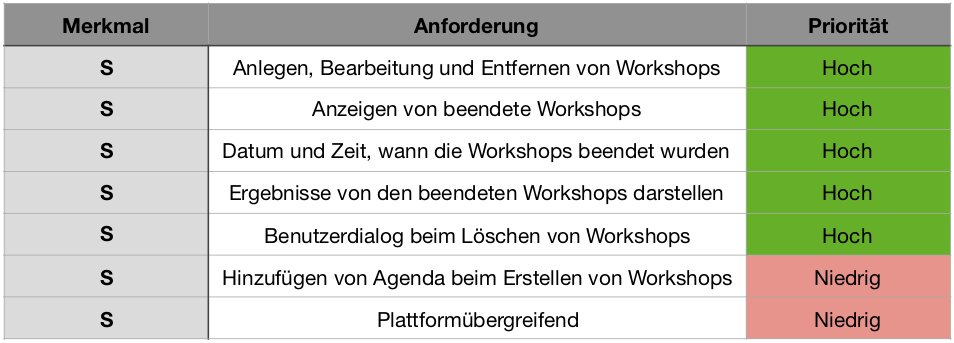
\includegraphics[scale=0.6]{img/Startseite.png}
  \caption{Muss- und Kann-Anforderungen für die Startseite (S)}
  \label{fig:startseite}
\end{figure}	

\begin{figure}[H]
  \centering  
  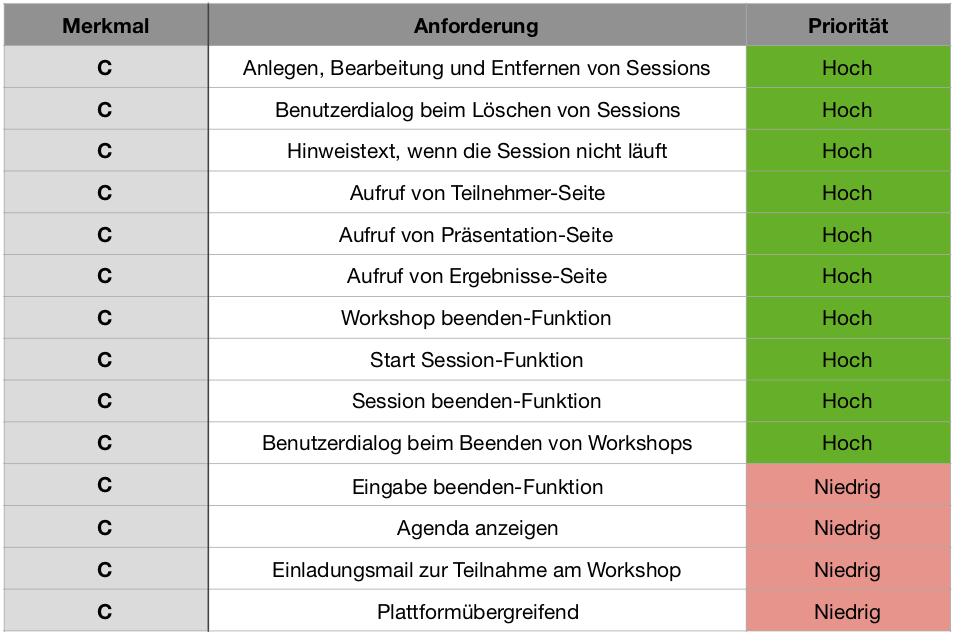
\includegraphics[scale=0.6]{img/Controller-Seite.png}
  \caption{Muss- und Kann-Anforderungen für die Workshop Controller-Seite (C)}
  \label{fig:controller-seite}
\end{figure}

\begin{figure}[H]
  \centering  
  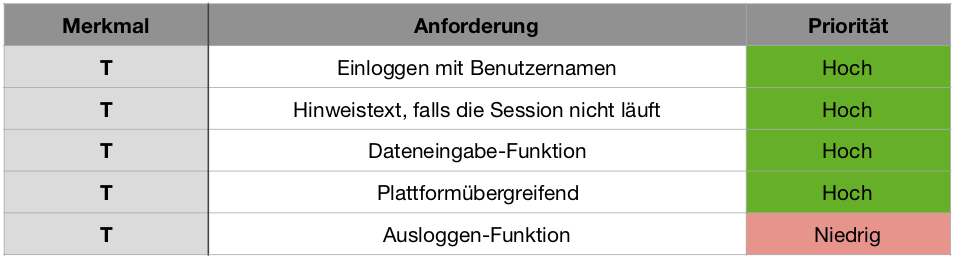
\includegraphics[scale=0.6]{img/Teilnehmer-Seite.png}
  \caption{Muss- und Kann-Anforderungen für die Teilnehmer-Seite (T)}
  \label{fig:teilnehmer-seite}
\end{figure}

\begin{figure}[H]
  \centering  
  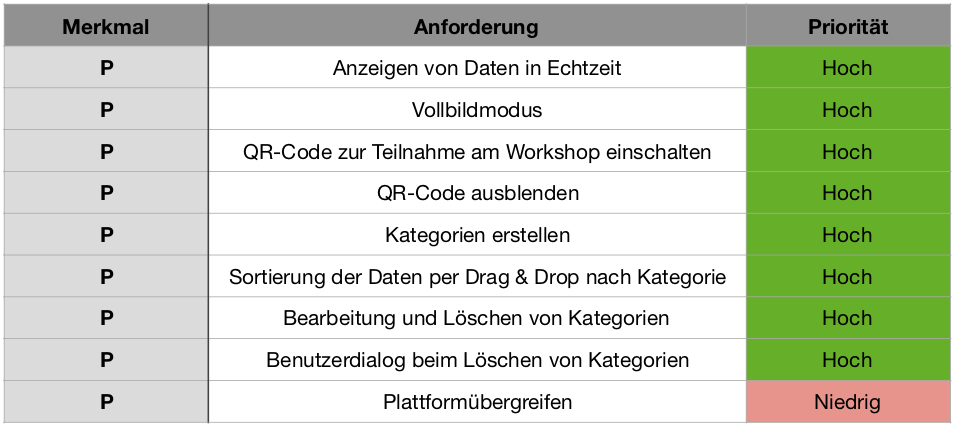
\includegraphics[scale=0.6]{img/Presentation-Seite.png}
  \caption{Muss- und Kann-Anforderungen für die Präsentation-Seite (P)}	
  \label{fig:presentation-seite}
\end{figure}

\begin{figure}[H]
  \centering  
  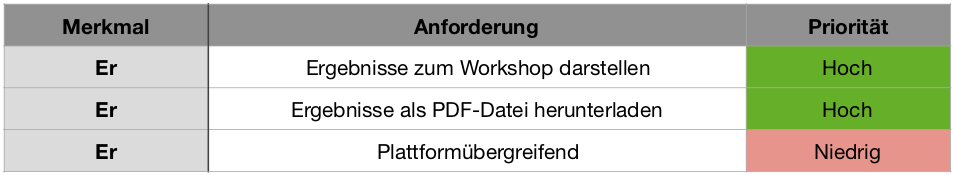
\includegraphics[scale=0.6]{img/Ergebnisse-Seite.png}
  \caption{Muss- und Kann-Anforderungen für die Ergebnisse-Seite (Er)}
  \label{fig:ergebnisse-seite}
\end{figure}

\begin{figure}[H]
  \centering  
  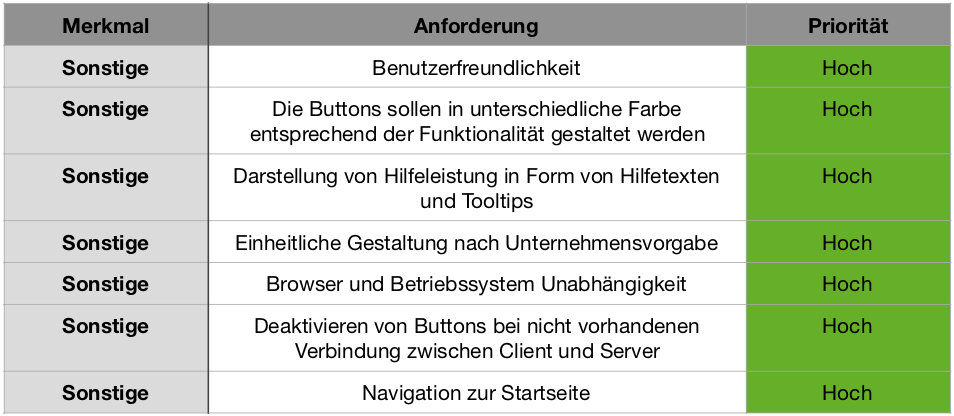
\includegraphics[scale=0.6]{img/Sonstige.png}
  \caption{Sonstige Muss- und Kann-Anforderungen für Webanwendung} 	
  \label{fig:sonstige}
\end{figure}

\subsection{Schematische Darstellung einer Bearbeitungshierarchie}
\begin{figure}[H]
  \centering  
  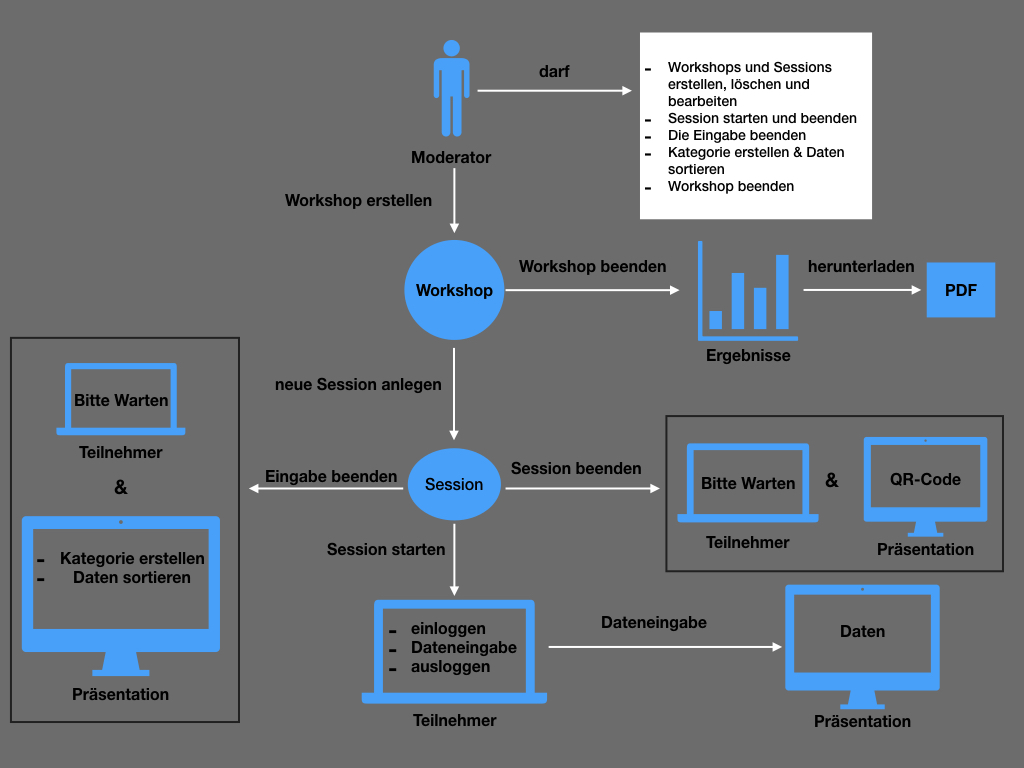
\includegraphics[scale=0.4]{img/Anforderung.jpeg}
  \caption{Darstellung der Bearbeitungshierarchie in der Webanwendung\newline [Quelle: eigene Abbildung]}
  \label{fig:anforderung}
\end{figure}













\chapter{Übersicht über die verwendete Webentwicklungswerkzeuge}
\label{cha:webentwicklungswerkzeuge}

\section{MidCom CMS}
\label{sec:midCom cms}

\section{HTML \& CSS}
\label{sec:html und css}

\section{Bootstrap}
\label{sec:bootstrap}

\section{PHP \& phpMyAdmin}
\label{sec:php und phpMyAdmin}

\section{Ajax}
\label{sec:Ajax}

\section{Javascript Framework jQuery}
\label{sec:jquery}

\subsection{jQuery UI}

\section{Recherche nach verwendbarer Technologie für die Kommunikation zwischen Client und Server}
\label{sec:kommunikation zwischen client und server}



%\chapter{Entwicklung der Sensorik}
\label{chap:entwicklung}


\section{Grobkonzept der Sensorik}
\label{sec:grobkonzept}

%\chapter{Ergebnisse}
\label{sec:ergebnisse}


%\chapter{Diskussion}
\label{sec:diskussion}

\section{Zusammenfassende Bewertung}
\label{sec:überschrift}

\section{Ausblick}
\label{sec:ausblick}

%Literaturverzeichnis
\bibliographystyle{unsrt}
\bibliography{Literatur}

\end{document}
